%%%%%%%%%%%%%%%%%%%%%%%%%%%%%%%%%%%%%%%%%%%%%%%%%%%%%%%%%%%%
%%  This Beamer template was created by Cameron Bracken.
%%  Anyone can freely use or modify it for any purpose
%%  without attribution.
%%
%%  Last Modified: January 9, 2009
%%

\documentclass[xcolor=x11names,compress, graphics]{beamer}

%% General document %%%%%%%%%%%%%%%%%%%%%%%%%%%%%%%%%%
\usepackage{graphicx}
\usepackage{tikz}
\usetikzlibrary{decorations.fractals}
%%%%%%%%%%%%%%%%%%%%%%%%%%%%%%%%%%%%%%%%%%%%%%%%%%%%%%
\usepackage{movie15}
\usepackage{float}
\usepackage{subfig}
\usepackage{amsmath}
\usepackage{amsfonts}
\usepackage{mathrsfs}
\usepackage{mathtools}

\usepackage{algorithm, algorithmic}

%% Beamer Layout %%%%%%%%%%%%%%%%%%%%%%%%%%%%%%%%%%
\useoutertheme[subsection=false,shadow]{miniframes}
\useinnertheme{default}
\usefonttheme{serif}
\usepackage{palatino}

\setbeamerfont{title like}{shape=\scshape}
\setbeamerfont{frametitle}{shape=\scshape}

\setbeamercolor*{lower separation line head}{bg=DeepSkyBlue4} 
\setbeamercolor*{normal text}{fg=black,bg=white} 
\setbeamercolor*{alerted text}{fg=red} 
\setbeamercolor*{example text}{fg=black} 
\setbeamercolor*{structure}{fg=black} 
 
\setbeamercolor*{palette tertiary}{fg=black,bg=black!10} 
\setbeamercolor*{palette secondary}{fg=black,bg=black!10}
\setbeamercolor*{palette quaternary}{fg=black,bg=black!10} 

%% Set the background and font color of the blocks 
\setbeamercolor{block title}{bg=DeepSkyBlue4,fg=white}

%% Set the type of the blocks
\setbeamertemplate{blocks}[shadow=true]

\newcommand{\topline}{%
  \tikz[remember picture,overlay] {%
    \draw[DeepSkyBlue4] ([yshift=-1.5cm, xshift = 1cm]current page.north west)
             -- ([yshift=-1.5cm,xshift=\paperwidth-1cm]current page.north west);}}
             
\setbeamertemplate{section in toc}[sections numbered]           

\renewcommand{\(}{\begin{columns}}
\renewcommand{\)}{\end{columns}}
\newcommand{\<}[1]{\begin{column}{#1}}
\renewcommand{\>}{\end{column}}

\usepackage[skip=10pt,font=scriptsize]{caption}
\captionsetup[figure]{labelformat=empty}

\DeclarePairedDelimiter\floor{\lfloor}{\rfloor}

\makeatother
\setbeamertemplate{footline}
{
  \leavevmode%
  \hbox{%
  \begin{beamercolorbox}[wd=.4\paperwidth,ht=2.25ex,dp=1ex,center]{author in head/foot}%
    \usebeamerfont{author in head/foot}\insertshortauthor
  \end{beamercolorbox}%
  \begin{beamercolorbox}[wd=.6\paperwidth,ht=2.25ex,dp=1ex,center]{title in head/foot}%
    \usebeamerfont{title in head/foot}\insertshorttitle\hspace*{3em}
    \insertframenumber{} / \inserttotalframenumber\hspace*{1ex}
  \end{beamercolorbox}}%
  \vskip0pt%
}
\makeatletter
%%%%%%%%%%%%%%%%%%%%%%%%%%%%%%%%%%%%%%%%%%%%%%%%%%

\title{\scshape \textbf{Divide And Conquer Paradigm}}
\author{\scriptsize\scshape Angel No\'e Mart\'inez Gonz\'alez}


\begin{document}

% The title page
\begin{frame}
\setcounter{framenumber}{1}
\titlepage
\scriptsize

\end{frame}
%===============


\section[\scshape Paradigm]{\scshape Paradigm}
\begin{frame}[allowframebreaks]{The Paradigm}
\topline

This paradigm solves a problem \textbf{recursively} applying three steps at each level of the recursion

\begin{itemize}
    \item \textbf{DIVIDE} the problem into a smaller sub-problems.
    \item \textbf{CONQUER} via recursive calls.
    \item \textbf{COMBINE} solutions of sub-problems into one of the original problem.
\end{itemize}

Consider also a \textbf{base case} for small enough sub-problems.

\framebreak
\topline

{\scshape\Large Insights and Hints}

\begin{itemize}
    \item Sub-problems can be any size: $1/2$, $1/3$, etc.
    \item Generally, third step is the key to achieve good performance.
    \item Base case is often too ingénue.
\end{itemize}

\framebreak
\topline


{\scshape\Large Merge sort (retake) }

\begin{minipage}{5cm}

\captionof*{algorithm}{}{{\scshape merge-sort}($A, p, r$)}
\begin{algorithmic}[1]
\IF{$p<r$}
	\STATE $q = \floor*{(p+r)/2}$
	\STATE {\scshape merge-sort}($A, p, q$)
	\STATE {\scshape merge-sort}($A, q, r$)
	\STATE {\scshape merge}($A, p, q, r$)
\ENDIF
\end{algorithmic}

\end{minipage}\ \ 
\begin{minipage}{5cm}

\captionof*{algorithm}{}{{\scshape merge}($A, p, q, r$)}
\begin{algorithmic}[1]
\STATE $B=1^{st}$ part of array.
\STATE $C=2^{nd}$ part of array.
\STATE $i=1,j=1$
\FOR{$k=1$ to $n$}
	\IF{$B[i]<C[j]$}
		\STATE $A[k]=B[i++]$
%		\STATE $i++$
	\ELSE
		\STATE $A[k]=C[j++]$
%		\STATE $j++$
	\ENDIF
\ENDFOR
\end{algorithmic}

\end{minipage}



\end{frame}

\section[\scshape Counting Inversions]{\scshape Counting Inversions}
\begin{frame}[allowframebreaks]{Counting Inversions}
\topline


\end{frame}

\section[\scshape The Maximum Subarray]{\scshape The Maximum Subarray}
\begin{frame}[allowframebreaks]{The Maximum Subarray}
\topline


\end{frame}

\section[\scshape Binary Search]{\scshape Binary Search}
\begin{frame}[allowframebreaks]{Binary Search}
\topline


\end{frame}


\section[\scshape Recurrence Tree]{\scshape Recurrence Tree}
\begin{frame}{Recurrence Tree}
\topline

{\scshape\Large Merge sort recursion tree}

\begin{figure}
	\begin{center}
		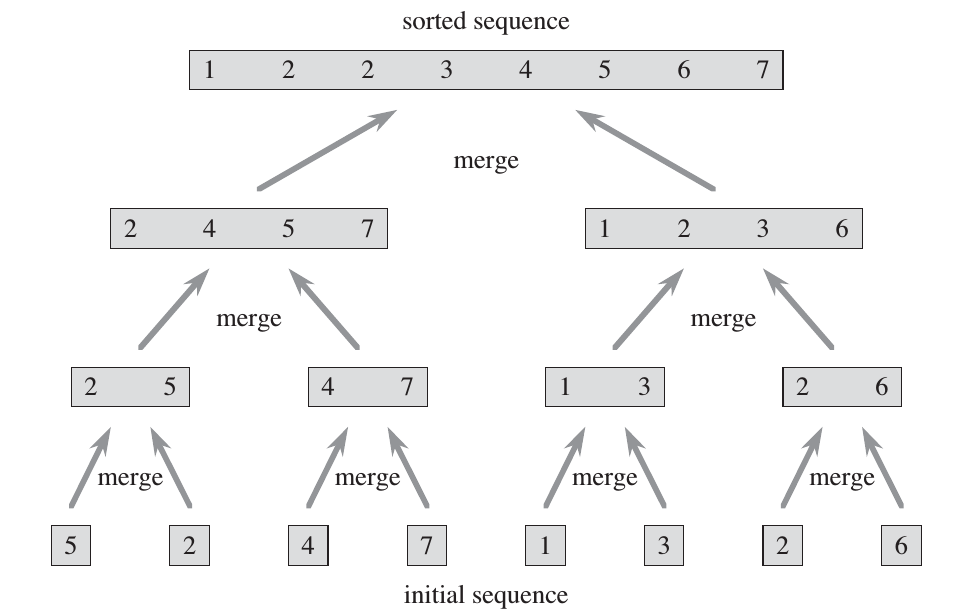
\includegraphics[width=8cm]{Figures/mergeSortTree.png}
	\end{center}
\end{figure}

At each level $j=0,1,...,log_2(n)$, there are $2^j$ subproblems of size $n/2^j$.

\end{frame}

\section[\scshape Master Method]{\scshape Master Method}
\begin{frame}[allowframebreaks]{The Master Method}
\topline

{\scshape\Large A black box }

\end{frame}

\end{document}